\subsection{Register Allocation}
\label{sec:register}
\begin{figure}[htbp]
\begin{center}
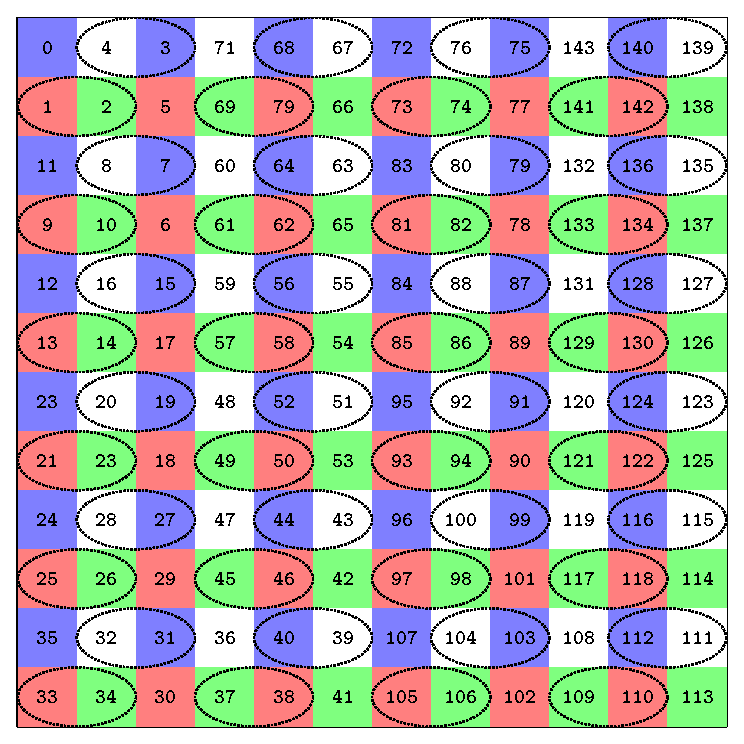
\includegraphics[scale=0.5]{reg}
\caption{Register allocation in SGEMM. The number in the cell is register index.
Different colors denote the mapping of register banks: green$\rightarrow$bank0,
    blue$\rightarrow$bank1, gray$\rightarrow$bank2, red$\rightarrow$bank3.}
\label{fig:reg}
\end{center}
\end{figure}

To allocate registers for $A$ column, $B$ row and $C$ sub-matrix as Algorithm~\ref{gemm}, we have three objectives: correctness, no bank conflict and tight register indices.
{\tt LDG.128} restricts $4$ words alignment for registers.
Since NVIDIA GPU does not have $128$-bit register, 
four consecutive $32$-bit registers {\tt RN}, {\tt RN+1}, {\tt RN+2}, and {\tt RN+3} will be an equivalence for 128 bit
register.
%a $128$-bit load instruction ({\tt LDG.128}) writes the data to four consecutive $32$-bit registers {\tt RN}, {\tt RN+1}, {\tt RN+2}, and {\tt RN+3} given one destination register $RN$.
% in order to use $128$-bit load, one destination register $RN$ is given,
% results will be written to
% four $32$-bit registers: {\tt RN}, {\tt RN+1}, {\tt RN+2}, {\tt RN+3}.
We discover an undocumented restriction that $N\%4=0$ to avoid illegal instruction error.
% It's not hard to understand this restriction,
The $4$ words alignment restriction for {\tt LDG.128} simplifies hardware logic and cuts down power.
Since we use {\tt LDG.128} to load $A$ and $B$, there are $2$ bank allocation choices limited by $N\%4==0$ restriction and Kepler's bank distribution (Table~\ref{tab:reg}).
We assume allocate $A$ matrix bank $\begin{bmatrix} 0 \\ 1  \end{bmatrix}$,
    $B$ bank $\begin{bmatrix} 2 & 3 \end{bmatrix}$ as shown in Figure~\ref{fig:reg}, 2 choices left for $C$,
$\begin{bmatrix} 1 & 2 \\ 3 & 0  \end{bmatrix}$ and
$\begin{bmatrix} 3 & 1 \\ 0 & 2  \end{bmatrix}$.
The $2\times2=4$ bank patterns for SGEMM are equivalent in performance, then we arbitrarily
choose $\begin{bmatrix} 0 \\ 1  \end{bmatrix}$ $\begin{bmatrix} 2 & 3 \end{bmatrix}$
    $\begin{bmatrix} 1 & 2 \\ 3 & 0  \end{bmatrix}$ for $A$, $B$ and $C$ respectively.
We use different colors to represent the four banks and show the register allocation when computing a $12 \times 12$ sub-matrix of C in Figure~\ref{fig:reg}.
% We have $2\times2$ bank patterns for SGEMM, these four patterns are equivalent in performance,
To allocate actual register index, we choose continuous register index so that register index do not get too big to exceed 255 restriction. 
It can be verified that every $C_{ij}$, $A_i$ and $B_j$ have different banks in Figure~\ref{fig:reg}, thus register bank conflicts are successfully avoided.
% for example $C_{01}$'s color is white, $A_0$'s color is green and $B_1$'s color is red, .
